\documentclass[unknownkeysallowed]{beamer}
\usepackage[french,english]{babel}
\usepackage{../sty/beamer_js}
\usepackage{../sty/shortcuts_js}


\newcommand{\Benchopt}{\texttt{Benchopt}}

\definecolor{tomcolor}{rgb}{0.,.3,.6}
\lstset{basicstyle=\color{tomcolor}\scriptsize\ttfamily}
\addbibresource{../biblio/biblio.bib}
\captionsetup[subfigure]{labelformat=empty}
\begin{document}

%%%%%%%%%%%%%%%%%%%%%%%%%%%%%%%%%%%%%%%%%%%%%%%%%%%%%%%%%%%%%%%%%%%%%%%%%%%%%%%
%%%%%%%%%%%%%%%%%%%%%%             Headers               %%%%%%%%%%%%%%%%%%%%%%
%%%%%%%%%%%%%%%%%%%%%%%%%%%%%%%%%%%%%%%%%%%%%%%%%%%%%%%%%%%%%%%%%%%%%%%%%%%%%%%


%%%%%%%%%%%%%%%%%%%%%%%%%%%%%%%%%%%%%%%%%%%%%%%%%%%%%%%%%%%%%%%%%%%%%%%%%%%%%%%
\begin{frame}
\bigskip
\bigskip
\begin{center}{
\LARGE\color{marron}
\textbf{\texttt{Benchopt}:\\
Reproducible, efficient and collaborative optimization benchmarks}
\textbf{ }\\
}

\color{marron}
\end{center}

\vspace{0.5cm}

\begin{center}
\textbf{Benchopt contributors} \\
\vspace{0.1cm}
\url{https://benchopt.github.io}\\
\end{center}

\centering

\includegraphics[width=0.43\textwidth]{../logo/benchopt_logo.pdf}

\end{frame}
%%%%%%%%%%%%%%%%%%%%%%%%%%%%%%%%%%%%%%%%%%%%%%%%%%%%%%%%%%%%%%%%%%%%%%%%%%%%%%%

%%%%%%%%%%%%%%%%%%%%%%%%%%%%%%%%%%%%%%%%%%%%%%%%%%%%%%%%%%%%%%%%%%%%%%%%%%%%%%%
\begin{frame}{Contributors from...}
Logos Inria, CNRS, Berkeley, Univ Luxembourg, Imag, Lund, Télécom, Criteo, Ulm, Imag ?
\end{frame}
%%%%%%%%%%%%%%%%%%%%%%%%%%%%%%%%%%%%%%%%%%%%%%%%%%%%%%%%%%%%%%%%%%%%%%%%%%%%%%%



%%%%%%%%%%%%%%%%%%%%%%%%%%%%%%%%%%%%%%%%%%%%%%%%%%%%%%%%%%%%%%%%%%%%%%%%%%%%%%%
\begin{frame}{Benchmarking algorithms is a pain}

Numerical validation is at the heart of Machine Learning.

Best methods are chosen

Doing a benchmark is a hassle:


% \begin{minipage}{.8\textwidth}
\begin{itemize}
	\item Takes time to reimplement methods
	\item Takes time for reviewers to check reimplementations
	\item Takes time to recode the tools needed
	\item All of this $\times$ yearly number of ML submissions
\end{itemize}
% \end{minipage}

\vskip2em


\Benchopt{} makes this effort \textbf{open}, \textbf{collaborative} and \textbf{easy}.

\end{frame}
%%%%%%%%%%%%%%%%%%%%%%%%%%%%%%%%%%%%%%%%%%%%%%%%%%%%%%%%%%%%%%%%%%%%%%%%%%%%%%%



%%%%%%%%%%%%%%%%%%%%%%%%%%%%%%%%%%%%%%%%%%%%%%%%%%%%%%%%%%%%%%%%%%%%%%%%%%%%%%%
\begin{frame}[fragile]{\texttt{benchopt}}

Doing a  benchmark for the $\ell_2$ regularized logistic regression with multiple solvers and datasets is now easy as calling:\\[1em]

\begin{lstlisting}[language=bash]
git clone https://github.com/benchopt/benchmark_logreg_l2
benchopt run ./benchmark_logreg_l2
\end{lstlisting}

\vskip1.5em
\includegraphics[width=.45\textwidth]{logreg_l2}
\hskip3ex
\includegraphics[width=.45\textwidth]{logreg_l2_1}

\end{frame}
%%%%%%%%%%%%%%%%%%%%%%%%%%%%%%%%%%%%%%%%%%%%%%%%%%%%%%%%%%%%%%%%%%%%%%%%%%%%%%%


%%%%%%%%%%%%%%%%%%%%%%%%%%%%%%%%%%%%%%%%%%%%%%%%%%%%%%%%%%%%%%%%%%%%%%%%%%%%%%%
\begin{frame}{\texttt{benchopt}}

\texttt{benchopt} can also compare the same algo in different languages.\\[1em]

Here is an example comparing PGD in: Python; R; Julia.\\[1em]
{\centering
\vskip.5em
\includegraphics[width=.65\textwidth]{lasso_3_languages}\\}

\end{frame}
%%%%%%%%%%%%%%%%%%%%%%%%%%%%%%%%%%%%%%%%%%%%%%%%%%%%%%%%%%%%%%%%%%%%%%%%%%%%%%%


%%%%%%%%%%%%%%%%%%%%%%%%%%%%%%%%%%%%%%%%%%%%%%%%%%%%%%%%%%%%%%%%%%%%%%%%%%%%%%%
\begin{frame}{Benchmark: principle}

A benchmark is a directory with:\\
\begin{itemize}
    \item An \lstinline+objective.py+ file with an \lstinline+Objective+
    \item A directory \lstinline+solvers+ with one file per \lstinline+Solver+
    \item A directory \lstinline+datasets+ with \lstinline+Dataset+ generators/fetchers
\end{itemize}
\vskip1em

\rem each objects above can be parametrized

\vskip1em

The \lstinline+benchopt+ client runs a cross product and generates a csv file + convergence plots like above.\\[.5em]
We expose easy way to select the \lstinline+objective/solver/dataset+ you want to run.
\end{frame}
%%%%%%%%%%%%%%%%%%%%%%%%%%%%%%%%%%%%%%%%%%%%%%%%%%%%%%%%%%%%%%%%%%%%%%%%%%%%%%%


%%%%%%%%%%%%%%%%%%%%%%%%%%%%%%%%%%%%%%%%%%%%%%%%%%%%%%%%%%%%%%%%%%%%%%%%%%%%%%%
\begin{frame}{Status}

Currently, benchmarks implementation available for:\\[.5em]
\begin{itemize}
	\item Least Square
	\item Non-Negative Least Square
	\item Lasso
	\item L1/L2 Regularized Logistic Regression
\end{itemize}

% \vskip1em
% Help appreciated: feel free to \underline{join} our effort to create reproducible benchmarks by adding new objectives/solvers/datasets!!!\\[1em]

\end{frame}
%%%%%%%%%%%%%%%%%%%%%%%%%%%%%%%%%%%%%%%%%%%%%%%%%%%%%%%%%%%%%%%%%%%%%%%%%%%%%%%


%%%%%%%%%%%%%%%%%%%%%%%%%%%%%%%%%%%%%%%%%%%%%%%%%%%%%%%%%%%%%%%%%%%%%%%%%%%%%%%
{
\usebackgroundtemplate{\includegraphics[width=\paperwidth]{wanted}}
\begin{frame}[plain]
\end{frame}
}
%%%%%%%%%%%%%%%%%%%%%%%%%%%%%%%%%%%%%%%%%%%%%%%%%%%%%%%%%%%%%%%%%%%%%%%%%%%%%%%


%%%%%%%%%%%%%%%%%%%%%%%%%%%%%%%%%%%%%%%%%%%%%%%%%%%%%%%%%%%%%%%%%%%%%%%%%%%%%%%
\begin{frame}{\texttt{benchopt}}
    \centering
    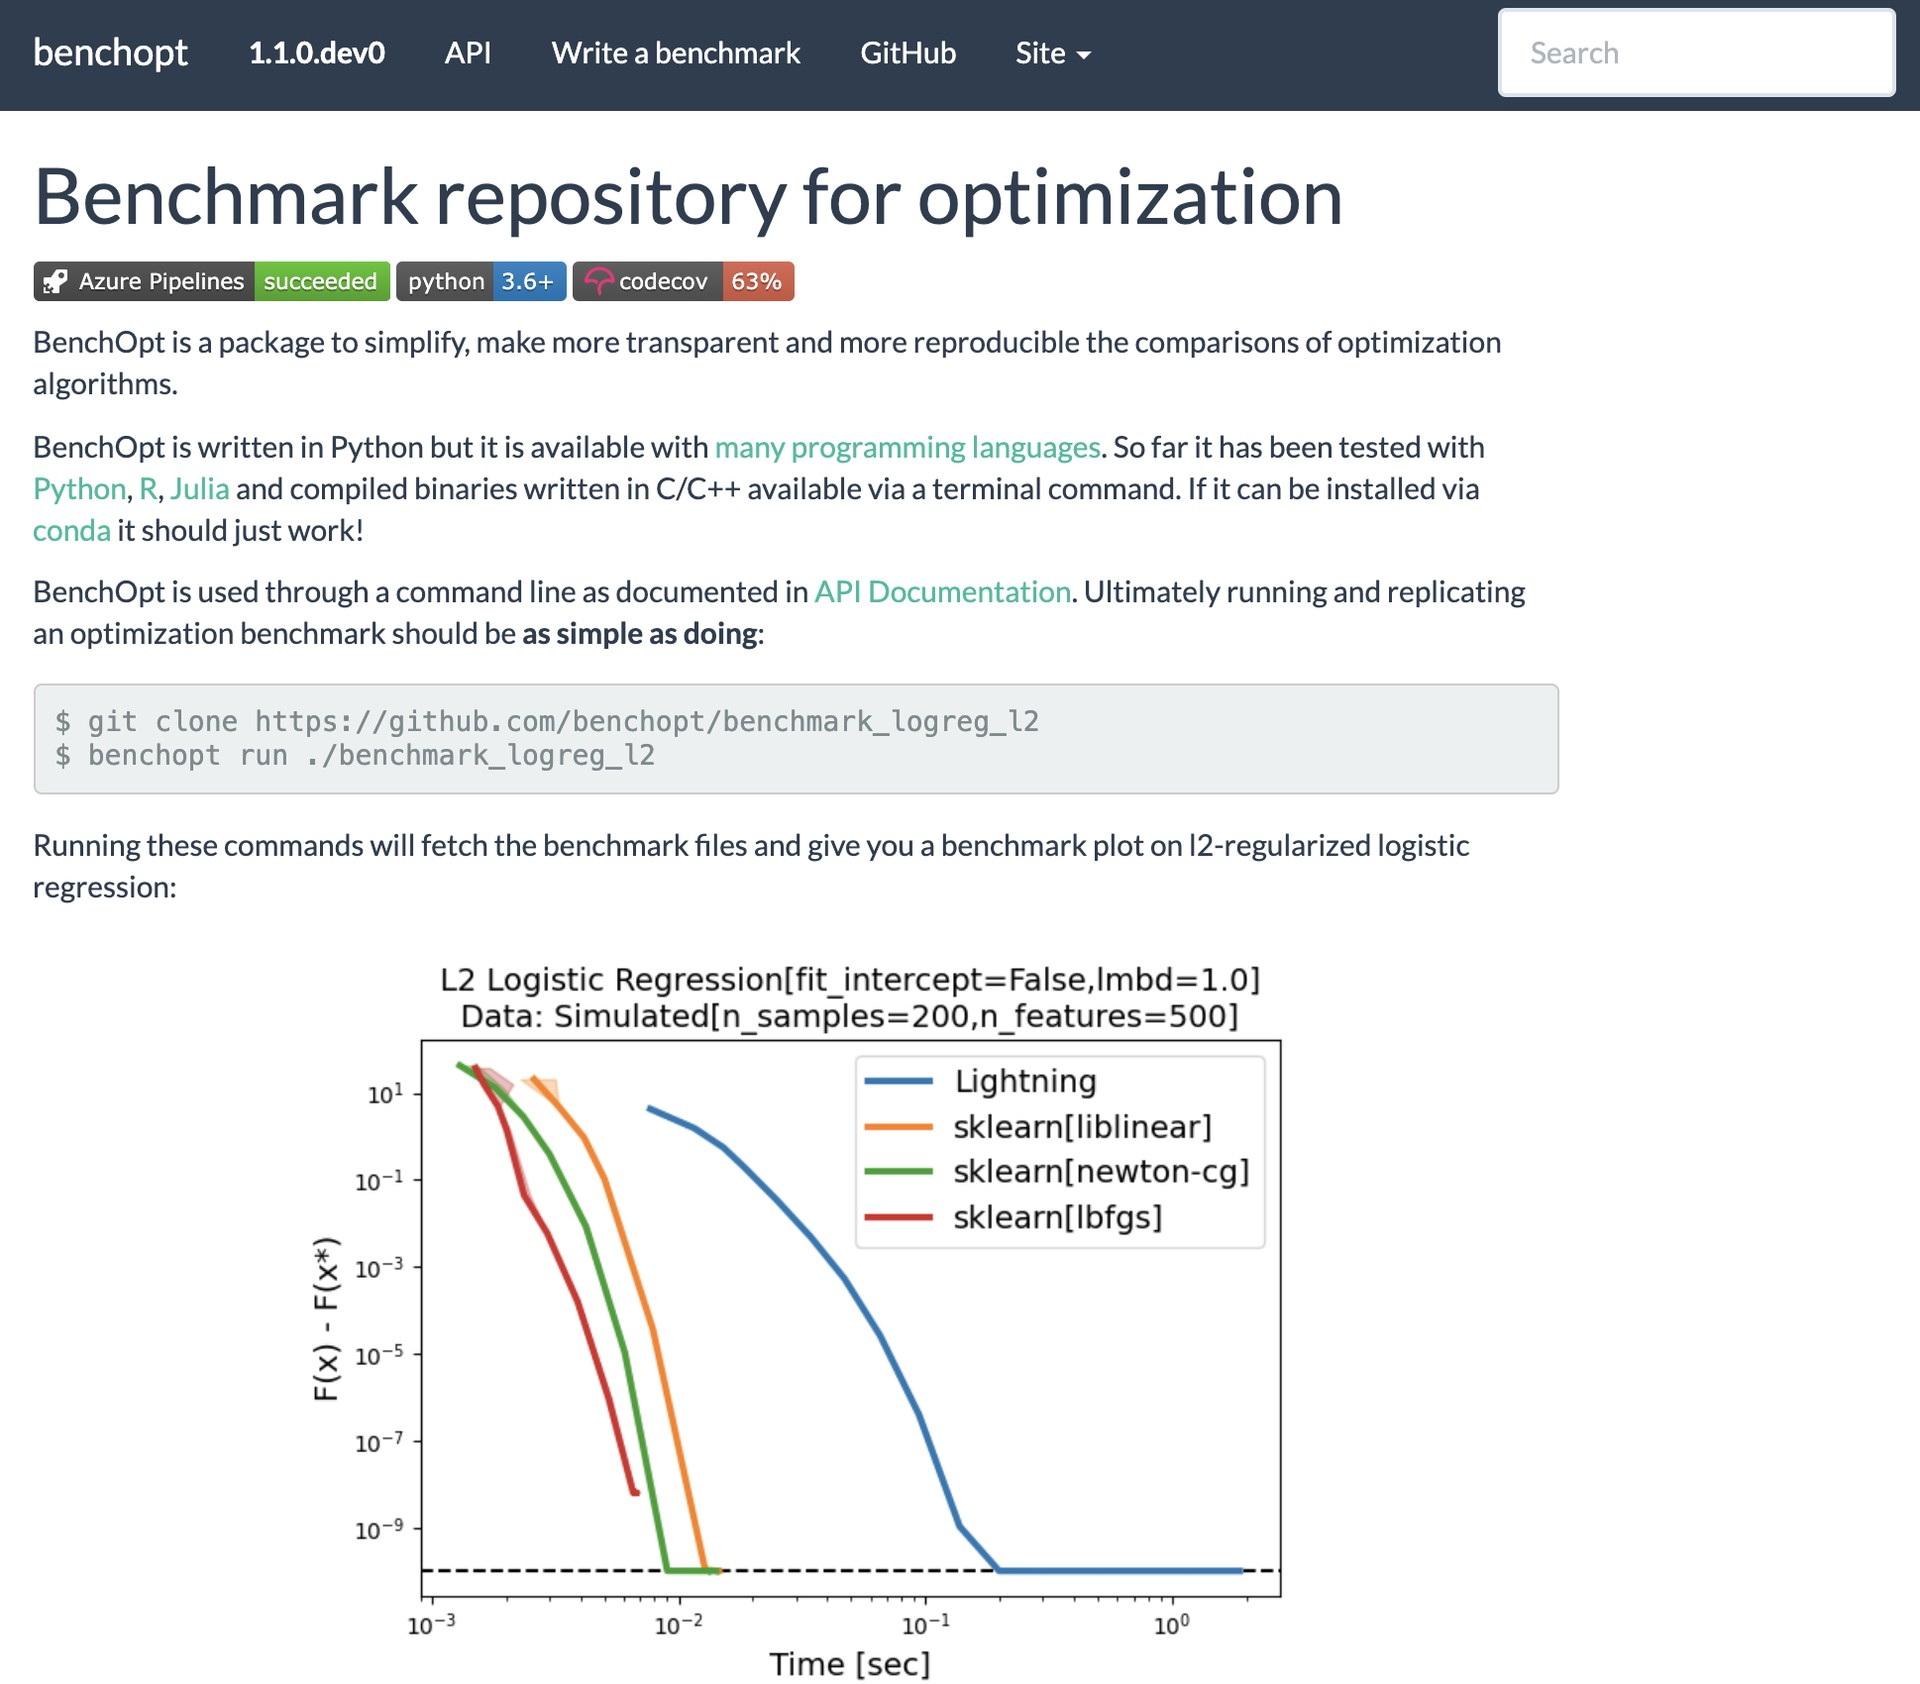
\includegraphics[width=.9\textwidth]{benchopt}\\
\end{frame}
%%%%%%%%%%%%%%%%%%%%%%%%%%%%%%%%%%%%%%%%%%%%%%%%%%%%%%%%%%%%%%%%%%%%%%%%%%%%%%%


%%%%%%%%%%%%%%%%%%%%%%%%%%%%%%%%%%%%%%%%%%%%%%%%%%%%%%%%%%%%%%%%%%%%%%%%%%%%%%%
\begin{frame}{Contact}

\vspace{0.4cm}
\centering
\includegraphics[width=0.93\textwidth]{contact_js}
\end{frame}
%%%%%%%%%%%%%%%%%%%%%%%%%%%%%%%%%%%%%%%%%%%%%%%%%%%%%%%%%%%%%%%%%%%%%%%%%%%%%%%



% %%%%%%%%%%%%%%%%%%%%%%%%%%%%%%%%%%%%%%%%%%%%%%%%%%%%%%%%%%%%%%%%%%%%%%%%%%%%%%%
% % Uncomment for references
% \begin{frame}{Bibliographie}
% \printbibliography
% \end{frame}
%  %%%%%%%%%%%%%%%%%%%%%%%%%%%%%%%%%%%%%%%%%%%%%%%%%%%%%%%%%%%%%%%%%%%%%%%%%%%%%%



\end{document}
